\documentclass[svgnames]{beamer}
\usepackage{mathabx}
\usepackage{mathrsfs}
%\usepackage{eulervm}
\usepackage{units}
\usepackage{calc}
\usepackage{tikz}
\usepackage[alpine]{ifsym}
\usepackage{marvosym}
\usepackage[normalem]{ulem}
\usepackage{braket}
\usepackage[matrix,arrow]{xy}
\usepackage{algorithm}
\usepackage{algorithmic}

\usetikzlibrary{arrows,automata,mindmap,patterns,shapes,snakes,trees}

\hypersetup{
	pdfkeywords={Restarting Automata, Tree Automata, Formal Languages,
		Restarting Tree Automata, Linear Context-Free Tree Languages},
	pdfpagemode={FullScreen}
}

\newtheorem*{proposition}{Proposition}

\mode<presentation>
{
	\usetheme{default}
	\usefonttheme[onlylarge]{structurebold}
	\usefonttheme[onlymath]{serif} % for Euler font
	
	%\setbeamertemplate{blocks}[rounded]
	\setbeamertemplate{navigation symbols}{}
	\setbeamertemplate{itemize items}{\textcolor{structure}{
		$\sqbullet$}}
	\setbeamertemplate{enumerate items}[square]
	%\setbeamertemplate{theorems}[numbered]
	\setbeamercolor{block title}{fg=structure,bg=gray!25}%
	\setbeamercolor{block body}{parent=normal text,bg=gray!10}%
	\setbeamercolor{block title example}{bg=gray!30!green!30}%
	\setbeamercolor{block body example}{parent=normal text,bg=gray!15!green!15}%
}

\title[TPM Emulator]{A Software-Based\\
	Trusted Platform Module Emulator}

\author[M. Strasser, H. Stamer]{
	\textbf{Mario Strasser}\inst{1}
	\and
	\underbar{\textbf{Heiko Stamer}}\inst{2}}

\institute[ETH Zurich, Uni Kassel]{
	\inst{1}
		ETH Zurich, Switzerland\\
		\texttt{strasser@tik.ee.ethz.ch}
	\and
	\inst{2}
		Universit{\"a}t Kassel, Germany\\
		\texttt{stamer@theory.informatik.uni-kassel.de}\\
		{\tiny\texttt{76F7 3011 329D 27DB 8D7C\quad  3F97 4F58 4EB8 FB2B E14F}}}

\date[TRUST 2008 (Villach)]{TRUST 2008, Scientific Conference on
	Trusted Computing\\
	Villach, Austria, March 11--12, 2008}

\subject{Trusted Computing}

% Falls eine Logodatei namens "university-logo-filename.xxx" vorhanden
% ist, wobei xxx ein von latex bzw. pdflatex lesbares Graphikformat
% ist, so kann man wie folgt ein Logo einf�gen:

\pgfdeclareimage[height=0.5cm]{university-logo}{uniklogo}
\logo{\pgfuseimage{university-logo}}

% Falls Aufz�hlungen immer schrittweise gezeigt werden sollen, kann
% folgendes Kommando benutzt werden:

%\beamerdefaultoverlayspecification{<+->}

\begin{document}

\begin{frame}
	\titlepage
\end{frame}

\begin{frame}
	\frametitle{Outline}
	\tableofcontents
\end{frame}

\logo{}
\renewcommand{\pause}{}

\section{Introduction}

\begin{frame}
	\frametitle{Why emulating a TPM in software?}
	TPM emulator has been proved to be useful in various ways, e.g.,
	\begin{itemize}
		\item to run more than one TPM instance per platform\\
			(\alert{\emph{virtualisation}}),
			\begin{itemize}
				\item Hewlett-Packard: Trustworthy Virtualisation Environment
			\end{itemize}
		\item to restore previously stored or artificially created states\\
			(\alert{\emph{testing}}, \alert{\emph{debugging}}, and 
			\alert{\emph{educational purposes}}),
			\begin{itemize}
				\item TU Graz: class ``AK IT-Sicherheit 1 / Trusted Computing''
				\item VMKnoppix (Xen Hypervisor)
			\end{itemize}
		\item to simulate new TPM commands and vendor extensions\\
			(\alert{\emph{research}} and \alert{\emph{development}})
			\begin{itemize}
				\item Princeton University, NEC, TI: energy and execution time
					analysis of ECC algorithms (DATE 2007)
				\item Nokia: Validation of MTM specification
			\end{itemize}
	\end{itemize}
	Of course, a software-based TPM cannot provide the same security
	guarantees (tamper-resistance, trust anchor) like a hardware chip.
\end{frame}

\begin{frame}
	\frametitle{Basic Facts}
	\begin{description}[]
		\item[Supported Operating Systems:] Linux, OpenBSD, FreeBSD, \ldots\\
			(packages for Gentoo Linux are available)
		\item[Last Stable Version:] 0.5.1 (2008-02-12), GPL v2,
			${}\approx 25$k LOC
		\item[Development Site:] \url{https://tpm-emulator.berlios.de/}
		\item[Third-Party Libraries:] GNU Multiple Precision Arithmetic Library
			(for bignum support)
		\item[History and Milestones:]\hfill\\
			\begin{itemize}
				\item 2004: Started by Mario Strasser as a semester thesis
				\item 2005: Identity functions and DAA support added
				\item 2006, December: Milestone version 0.5 released
			\end{itemize}
	\end{description}
\end{frame}

\section{Design and Implementation}

\begin{frame}
	\frametitle{Design and Implementation}
	\begin{description}[]
		\item[New Design:] User-space daemon \texttt{tpmd}
			(since version 0.5)\\
			\begin{center}
				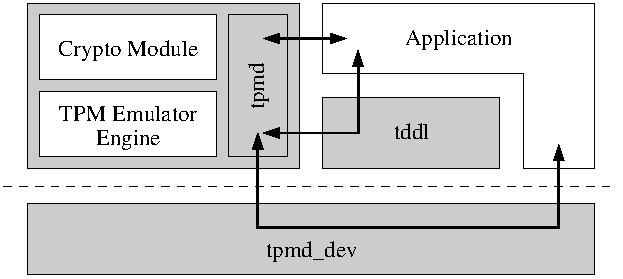
\includegraphics[width=.95\textwidth]{figures/system_overview}
			\end{center}
		\item[Accessing the Emulator:]\hfill\\
			{\small\begin{enumerate}
				\item Direct (Unix domain socket \texttt{/var/run/tpm/tpmd\_socket:0})
				\item Recommended (TDDL interface according to TSS spec.)
				\item Legacy (Linux/BSD kernel modul \texttt{tmpd\_dev} provides
					\texttt{/dev/tmp})
			\end{enumerate}}
	\end{description}
\end{frame}

\section{Performance Evaluation}

\begin{frame}
	\frametitle{Performance Evaluation}
\end{frame}

\section{Compliance Tests}

\begin{frame}
	\frametitle{Compliance Tests}
\end{frame}

\section{Conclusion}

\begin{frame}
	\frametitle{Conclusion}
	\begin{description}[]
		\item[Roadmap:]\hfill\\
			\begin{enumerate}
				\item Provide autoconf/automake support
				\item Complete missing mandatory TPM commands
				\item Support other operating systems
			\end{enumerate}
	\end{description}
\end{frame}

\begin{frame}
	\frametitle{}
	\pause
	\begin{center}
		\begin{Huge}
			\textbf{Thank you! Questions?}
		\end{Huge}
	\end{center}
\end{frame}

\section*{References}

\begin{frame}
	\frametitle{References}
	{\tiny\begin{thebibliography}{999999}
		%\beamertemplatetextbibitems
	\beamertemplatebookbibitems
		\bibitem{Mitchell2005}
			Chris Mitchell et~al.
			\newblock Trusted Computing.
			\newblock IET, 2005.
		\bibitem{Challener2008}
			David Challener, Kent Yoder, Ryan Catherman, David Safford, and
			Leendert Van Doorn.
			\newblock A Practical Guide to Trusted Computing.
			\newblock IBM Press, 2008.
		\bibitem{TPM}
			Trusted Computing Group.
			\newblock TPM Specification, Version 1.2, Revision 103.
			\newblock
			{\large\Keyboard}\hspace{2mm}\url{https://www.trustedcomputinggroup.org/specs/TPM/}.
	\beamertemplatearticlebibitems
		\bibitem{Sadeghi}
			Ahmad-Reza Sadeghi, Marcel Selhorst, Christian St\"{u}ble,
			Christian Wachsmann, and Marcel Winandy.
			\newblock TCG inside? A Note on TPM Specification Compliance.
			\newblock Proceedings of STC '06, pp. 47--56, 2006.
	%\beamertemplatetextbibitems
		\bibitem{TPMEmu}
			Mario Strasser et~al.
			\newblock Software-Based Trusted Platform Module Emulator.
			\newblock
			{\large\Keyboard}\hspace{2mm}\url{http://tpm-emulator.berlios.de/}.
		\bibitem{jTSS}
			TU Graz, IAIK.
			\newblock jTSS -- Java TCG Software Stack.
			\newblock
			{\large\Keyboard}\hspace{2mm}\url{http://trustedjava.sourceforge.net/}.
		\bibitem{trousers}
			Kent Yoder et~al.
			\newblock TrouSerS -- Open-source TCG Software Stack.
			\newblock
			{\large\Keyboard}\hspace{2mm}\url{http://trousers.sourceforge.net/}.
		\bibitem{ibmdaatest}
			Roger Zimmermann.
			\newblock IBM Direct Anonymous Attestation Tools -- TPM Test Suite.
			\newblock
			{\large\Keyboard}\hspace{2mm}\url{http://www.zurich.ibm.com/security/daa/}.
	\end{thebibliography}}
\end{frame}

\end{document}
